\documentclass{beamer}


\usepackage[frenchb]{babel}

\usepackage[T1]{fontenc}
%\usepackage[latin1]{inputenc}
\usepackage[utf8]{inputenc}

\usepackage{marvosym}



\newcommand{\be}[1]{ \begin{equation} \label{#1}}
\newcommand{\ee}{\end{equation}}


\newcommand{\bes}[1]{ \begin{equation} \label{#1}\begin{array}{rl}}
\newcommand{\ees}{\end{array}\end{equation}}


\usepackage[normalem]{ ulem }
\usepackage{soul}

% \usetheme{default} -> A utiliser dans un premier temps

% \usetheme{Warsaw} -> A utiliser dans un second temps


\usepackage{amsmath} % AMS Math Package
\usepackage{amsthm} % Theorem Formatting
\usepackage{amssymb} % Math symbols such as \mathbb
\usepackage{graphicx} % Allows for eps images
\usepackage{multicol} % Allows for multiple columns
\usepackage[dvips,letterpaper,margin=1in,bottom=1in]{geometry}
\usepackage{hyperref}
\usepackage{mathrsfs}
\usepackage{amsmath,amscd}
\usepackage[all,cmtip]{xy}
\usepackage{bbm}
%%%%%%%%%%%%%%%%%%%%%%%%%%%%%%%%%%%%%%%%%%%%%%%%%%%
%COLOR PACKEGE
\usepackage{color}
	\definecolor{red}{RGB}{255,0,0}
	\definecolor{blue}{RGB}{30, 144, 255}
	\definecolor{black}{RGB}{0, 0, 0}	
	\definecolor{mygreen}{RGB}{28,172,0} % color values Red, Green, Blue
	\definecolor{mylilas}{RGB}{170,55,241}
%%%%%%%%%%%%%%%%%%%%%%%%%%%%%%%%%%%%%%%%%%%%%%%%%%%
\usepackage{menukeys}
\usepackage{framed}
\renewmenumacro{\directory}{pathswithfolder} % default: paths
%%%%%%%%%%%%%%%%%%%%%%%%%%%%%%%%%%%%%%%%%%%%%%%%%%%
%MATLAB

\usepackage{listings}
\lstset{language=Matlab,%
    %basicstyle=\color{red},
	%basicstyle=\ttfamily,frame=single,xleftmargin=3em,xrightmargin=3em  
	frame=single,xleftmargin=2em,%xrightmargin=2em,    
    breaklines=true,%
    morekeywords={matlab2tikz},
    keywordstyle=\color{blue},%
    morekeywords=[2]{1}, keywordstyle=[2]{\color{black}},
    identifierstyle=\color{black},%
    stringstyle=\color{mylilas},
    commentstyle=\color{mygreen},%
    showstringspaces=false,%without this there will be a symbol in the places where there is a space
    numbers=left,%
    numberstyle={\tiny \color{black}},% size of the numbers
    numbersep=9pt, % this defines how far the numbers are from the text
    emph=[1]{for,end,break},emphstyle=[1]\color{red}, %some words to emphasise
    %emph=[2]{word1,word2}, emphstyle=[2]{style}, 
}
%%%%%%%%%%%%%%%%%%%%%%%%%%%%%%%%%%%%%%%%%%%%%%%%%%%
%\lstinputlisting{*.m} for using
%\usepackage[framed,numbered,autolinebreaks,useliterate]{mcode}
%%%%%%%%%%%%%%%%%%%%%%%%%%%%%%%%%%%%%%%%%%%%%%%%%%%
%MACROS
\newcommand{\ti}[1]{\textit{#1}}


\newcommand{\ssp}{\vspace{.2cm} }

\title{A (kind of) practical review on global stability approches}

\subtitle{}

\author{D. Fabre}

\institute{IMFT, groupe InterfaceS}

\date{Informal Workshop "D\&D", 10 juillet 2018}


\AtBeginSection{
\frame{\tableofcontents[current]}
}


\begin{document}


\begin{frame}

\titlepage

\end{frame}

\section{Linear global stability  : basic principles, and a few useful tricks}

\subsection{Qu'es aquò ??}

\begin{frame}{Qu'es aquò ?? } 


Instability problems are ubiquous in fluid mechanics

\ssp

Numerical resolution of such problems resorts to a specific class of numerical methods, which replace
time-stepping of the full equations by  assumptions about temporal dependance (modal expansion, amplitude equations, etc...)
 
 \ssp These methods are complementary to direct numerical resolution methods (i.e. time-stepping).

%Leur résolution fait appel à une classe de méthodes numériques spécifiques, 
%complémentaires aux approches de simulation directe, qui sont actuellement en plein développement. 

\ssp

We refer to {\em global stability} when the geometry requires resolution in 2 (or 3) spatial dimensions.


%On parle {\em stabilité globale} quand la géométrie du problème necésssite une résolution en 2D (ou en 3D).

\ssp

(as opposed to {\em local stability } which takes advantage of invariance directions (parallel flow, etc...)
to bring the problem to spatially 1D).
 

%(par opposition à {\em stabilité locale} quand des directions d'invariance (écoulement parallèle par ex.) permettent de rammener le problème à une résolution en 1D).


\end{frame}



%\subsection{Step 0 : computation of a base flow}

\begin{frame}{Base flow}

We look for a steady base-flow $({\bf u}_b;p_b)$ satisfying the steady Navier-Stokes equations, i.e. 
$NS ({\bf u}_b,p_b) = 0$.


Suppose that we have a 'guess' for the base flow $[{\bf u}_b^g,p_b^g]$  which almost satisfies the equations.  We look for a better approximation under the form
\be{Newton1}
[{\bf u}_b,p_b]  = [{\bf u}_b^g,p_b^g] + [\delta {\bf u}_b, \delta p_b] = 0.
\ee

Injecting into the Navier-Stokes equation lead to $$
NS ({\bf u}_b^g,p_b^g) + NSL_{{\bf u}_b^g}(\delta {\bf u}_b,\delta p_b)$$


Where $NSL$ is the linearised Navier-Stokes operator. 
%defined by its action on a flow field $({\bf u} ; p)$ as follows 



=>  matricial problem with the form $A \cdot \delta X = Y$. The procedure of Newton iteration is to solve iteratively this set of equations up to convergence.

\end{frame}




%\subsection{Step 1 : Eigenvalue computation}

\begin{frame}{Linear stability}

\be{startmodepropre}
{\bf u} = {\bf u}_b + \epsilon \hat{\bf u} e^{\lambda t} 
\ee

The eigenmodes is governed by the linear problem 
$$\lambda \hat{{\bf u}} = NSL_{{\bf u}_b}( \hat{\bf u},\hat{p})$$,

After discretization we end up with an eigenvalue problem with the matricial form
\be{Eigen_matricial}
\lambda B \hat{X} = A \hat{X}
\ee

\ssp
Iterative method : single-mode shift-invert iteration
$$
X^{n} =  (A- \lambda_{shift} B)^{-1} B X^{n-1}
$$ 

Generalization : Arnoldi

\end{frame}


%\subsection{Adjoint eigenmodes and structural sensitivity} 

\begin{frame}{Adjoint problem}

\small

Define a scalar product :
$$
\left< \phi_1, \phi_2 \right> = \int_\Omega \overline{\phi_1} \cdot \phi_2   \mbox{ d} \Omega
$$


We can first define the {\em adjoint linearised Navier-Stokes operator} $NSL^\dag$ defined by the property:
\bes{NSLAdj}
\forall ( {\bf u}, p ; {\bf u}^\dag, p^\dag), & \left< NSL^\dag_{\bf U}( {\bf u}^\dag,p^\dag) ,{\bf u}\right> + \left< \nabla \cdot {\bf u}^\dag,p\right>  \\
=& \left<{\bf u}^\dag, NSL_{\bf U} ({\bf u},p)\right> + \left< p^\dag, \nabla \cdot {\bf u}\right>.
\ees
We can then define the adjoint eigenmodes as the solutions to the eigenvalue problem 
\be{EigenAdj} 
\forall ( {\bf u}, p), \quad  \lambda^\dag \left< \hat{{\bf u}^\dag}, {\bf u}\right> =
 \left< NSL^\dag_{\bf U}( \hat{\bf v},\hat{p^\dag}) ,{\bf u}\right> + \left< \nabla \cdot \hat{\bf u}^\dag,p\right>  
\ee

Matricial form :

\be{Eigen_Adj_matricial}
\overline{\lambda}^\dag B \hat{X}\dag = A^T \hat{X}\dag.
\ee


\end{frame}

\begin{frame}{Adjoint mode and structural sensitivity}


Significance of the adjoint mode : 

(optimal perturbation)

\ssp
%\pause


%Structural sensitivity:

The adjoint eigenmode also allows us to introduce the so-called {\em structural sensitivity tensor } that is defined as 
\be{Structursens} 
{\bf{S}}({\bf{x}}) = \frac{|| \hat{\bf u}^\dag|| \,\, ||\hat{\bf u}|| }{{\left<\hat{\bf u}^\dag, \hat{\bf u}\right>}},
\ee 
which has became popular in the recent years.



\end{frame}

\subsection{Three ideas to really speed up your linear stability computations !}

\begin{frame}{Three ideas to really speed up your stability computations !}

\begin{itemize}[<+->]

\item Use simple shift-invert for computing a single mode !

\item Adapt your mesh !
\begin{itemize}
\item to base flow,
\item to base flow + eigenmode, 
\item to base flow + structural sensitivity !
\end{itemize}


\item Escape the real world : go into complex plane ! 

\begin{itemize}
\item Incompressible case : to handle strongly convective instabilities

(example : whisling jet, with Vincenzo Citro \& Raffaele Longobardi)

\item Compressible case : to handle non-reflective boundary conditions

(example : cylinder wake ; with Javier Sierra)
\end{itemize}


\end{itemize}

\end{frame}



%%%%%%%%%%%%%%%%%% CHAPTER 2 %%%%%%%%%%%%%%%%%%%%%%%%%%%
\section{StabFem : a software that may save your life !}
\subsection{Qu'es aquò ???}

%\subsection{StabFem : présentation du logiciel}



\begin{frame}{FreeFem++}

Finite element methods are well suited to global stability problerms.

The {\em FreeFem++} software is gaining popularity in the hydrodynamic stabillity community.
 %un outil très populaire dans la communauté de la stabilité hydrodynamique.

\small

\begin{itemize}[<+->]
%{\color{green} \Smiley{} \quad }  (solides, fluides, thermique, etc...)
\item
{\color{green} \Smiley{} \quad } Simple and intuitive syntax directly based on weak formulation.
%Syntaxe intuitive basée directement sur la formulation faible.
\item
{\color{green} \Smiley{} \quad } Powerful and adaptative mesh  (movemesh, adaptmesh, etc...)
% Mailleur puissant et adaptatif (movemesh, adaptmesh, etc...)
\item
{\color{green} \Smiley{} \quad } 2D and 3D.
\item
{\color{green} \Smiley{} \quad } Large choice of sequencial and parallel solvers  (Mumps, Petsc/Slepc, ..)
%Grand choix de solveurs séquentiels ou parallèles (Mumps, Petsc/Slepc, ..)
\item
{\color{red} \Frowny{} \quad } Limited graphical interface (ffglut) %Interface graphique limitée (ffglut).
\item
{\color{red} \Frowny{} \quad } Interpreted language : not suited to functional programming (but powerful macros).
%Language interprété : pas adapté à la programmation fonctionnelle (mais des macros puissantes).
\item
{\color{red} \Frowny{} \quad } Syntax may be touchy and debugging sometimes awkward...
%Syntaxe "chatouilleuse" et débuggage parfois complexe...
\end{itemize}
\end{frame}

\begin{frame}{Why interface FreeFem++ with another software ?}

\small

\begin{itemize}[<+->]

\item %Stratégie avant "StabFem" (2010-2017) :
Previous strategy :

Computation chain : freefem solvers / shell scripts / postprocessing with tecplot/gnuplot...

%Chaine de calcul : Solveurs FreeFem++ / Scripts Shell / Post-traitement Tecplot / Gnuplot.... 

%=> 50 programmes quasiment identiques + 10 manières d'effectuer le post-traitement,

%on ne s'y retrouve plus... 

=> 50 almost identical programs + 10 ways to handle post-processing => getting crazy !

\ssp 

\item %Nécessité d'une surcouche "driver"  pour piloter les calculs et tracer les résultats en mode "terminal" ou par l'intermédiaire de scripts.
=> Necessity of a  set of "drivers" in a high-level language to monitor computations and draw the results in "command-line" or "script" mode.


\item 
%Philosophie (à terme) : 1 travail (1 article) = 1 unique script Matlab pour reproduire tous les calculs et générer toutes les figures 
Philosophy (objective) : one work (one paper) = 1 unique program to generate all results and produce all figures.
(cf. Basilisk...)


%\item Choix actuel  : Drivers en Matlab/Octave


\end{itemize}


\end{frame}


%%%%%%%%%%%%%%%%%%%%%%%%%%%%%%%%%%%%%%%%%%%%%%%%
\begin{frame}{StabFem : Cahier des charges }
%Equations : 
%\begin{equation}
%$$\frac{\partial V }{\partial t} = \nu \frac{\partial^2 V}{\partial y^2} $$
%\label{eq:navier}
%\end{equation}
%(on a supposé pour simplifier qu'il n'y avait pas de gradient de pression autre qu'hydrostatique).
%Conditions limites : $\left. v\right|_{y=0} = 0$, $\left. v\right|_{y=h} = U(t)$  

\begin{itemize}[<+->]

\item StabFem : an open-source and easy-to-use software allowing a large range of computations in fluid mechanics.

\item Designed for both research  \& education.

\item Initially  oriented towards Global Stability Approches (Linear \& Nonlinear) but actually allowing a larger number of computations
(DNS, linear acoustics, etc...)

\item Multi-platform (Unix, MacOs, Windows) and designed to run on "light" computers (Laptops...)

\item Easy to use/install, 


\item Easy to customize to a variety of cases (incompressible, compressible, fixed/free objects, free surfaces,...)

\item Freeware, based on two softwares : FreeFem++ and \sout{Matlab}/{\color{red}Octave }

\item Developed as a collaborative project
(IMFT, Università di Salerno, ONERA, UPFL, ...)

\item Maintained on Github

\ssp
{\color{orange}
\verb! https://github.com/erbafdavid/StabFem !
}

\end{itemize}

\end{frame}





%%%%%%%%%%%%%%%%%%%%%%%%%%%%%%%%%%%%%%%%%%%%%%%%%%%%%%%%%%%%%%%%%%%%%%%%%%
\begin{frame}{Articulation FreeFem / Matlab}

\scriptsize

\begin{itemize}[<+->]

\item 
Etage 1 : Solveurs FreeFem++ "briques de base".

Un solveur par "classe de problèmes" (2D incompressible, 2D compressible, Axisymétrique incompressible...) et par "type de calcul" (calcul d'un champ de base, stabilité linéaire, ...)


\item  Etage 2 : drivers Matlab "génériques"  

Un unique driver pour chaque "type de calcul" , le choix du bon solveur est fait en fonction 
des paramètres optionnels fournis au driver.
  

  
\item Etage 3 : Les boucles sur les paramètres et la génération des figures sont faites dans un "script principal".

\item Les solveurs et les drivers génériques sont dans des répertoires communs {\bf SOURCES\_MATLAB/} et {\bf SOURCES\_FREEFEM/}, 

\item Les programmes spécifiques à chaque cas d'étude sont dans un répertoire spécifique.

Exemple : le répertoire "CYLINDRE" contient les programmes suivants :

\begin{enumerate}
\scriptsize
\item Mesh\_Cylinder.edp		\qquad -> Génération du maillage

\item Macros\_StabFem.edp \qquad -> Macros case-dependant (conditions limites et post-traitement)   

\item SCRIPT\_CYLINDER.m $\qquad$ -> Script "Maitre".

\end{enumerate}
\end{itemize}
\pause 


{\em Remarques : les programmes FreeFem doivent pouvoir être utilisés directement en dehors du driver StabFem, 
notamment pour faciliter le développement/débuggage...)}  

\ssp 

{\em Les contributeurs "utilisateurs" (ex. étudiant M1/M2) ne travaillent qu'à l'étage 3 et ne devraient travailler que sur ces 3 fichiers.
\ssp

Les contributeurs "développeurs" travaillent aux étages inférieurs...}


\end{frame}




\begin{frame}{Format d'échange des données}

\begin{itemize}[<+->]


\item Format de fichier d'échange ".ff2m", généré par FreeFem++ et relu par Matlab
 
\item Example d'en-tête d'un fichier .ff2m :

\lstinputlisting[linerange={1-4}]{../EXAMPLE_Lshape/Data.ff2m}
 
Ligne 4 : "TypeField1 NameField1 TypeField2 NameField2... "
  
TypeField can be "real" (scalar data), "real.N" (vectorial data), "P1" (data associated to mesh), ... 

\item Le fichier est lu et importé sous forme d'une {\em structure matlab}   

\item Illustration : cas "EXAMPLE\_Lshape"

\end{itemize}


\end{frame}



%\section{Using StabFem for Linear stability }

\subsection{Demonstration for the wake of a cylinder}

\begin{frame}{First step : Generation of a mesh and "guess" base flow}

\small

%\begin{lstlisting}
%bf=SF_Init('Mesh_Cylinder.edp', [-40 80 40]);
%\end{lstlisting}

\keys{bf=SF\_Init('Mesh\_Cylinder.edp', [-40 80 40]);}

\ssp

What the \keys{SF\_Init} driver does :

\begin{itemize}[<+->]
\item Runs the relevant FreeFem++ program \keys{Mesh\_Cylinder.edp}  with the corresponding parameters (here size of the domain),

{\scriptsize This program generates the following output files : \keys{mesh.msh} (mesh data), \keys{mesh.ff2m} (mesh information), \keys{SF\_Init.ff2m} (auxiliary information), \keys{BaseFlow\_init.txt} and \keys{BaseFlow\_init.ff2} ("guess" base flow).}


\item Reads all the output files,

\item Returns a matlab "structure" object containing all the data needed for post-processing and subsequent usage.
 
\end{itemize}

\end{frame}


%\subsection{Step 0 : computation of a base flow}

\begin{frame}{Computation of a Base flow : principle}

We look for a steady base-flow $({\bf u}_b;p_b)$ satisfying the steady Navier-Stokes equations, i.e. 
$NS ({\bf u}_b,p_b) = 0$.


Suppose that we have a 'guess' for the base flow $[{\bf u}_b^g,p_b^g]$  which almost satisfies the equations.  We look for a better approximation under the form
\be{Newton1}
[{\bf u}_b,p_b]  = [{\bf u}_b^g,p_b^g] + [\delta {\bf u}_b, \delta p_b] = 0.
\ee

Injecting into the Navier-Stokes equation lead to $$
NS ({\bf u}_b^g,p_b^g) + NSL_{{\bf u}_b^g}(\delta {\bf u}_b,\delta p_b)$$


Where $NSL$ is the linearised Navier-Stokes operator. 
%defined by its action on a flow field $({\bf u} ; p)$ as follows 



=>  matricial problem with the form $A \cdot \delta X = Y$. The procedure of Newton iteration is to solve iteratively this set of equations up to convergence.

\end{frame}




\begin{frame}{Computation of a Base flow : implementation}

\small



\keys{bf=SF\_BaseFlow(bf,'Re',10);}

%\begin{lstlisting}
%baseflow=SF_BaseFlow(baseflow,'Re',10);
%\end{lstlisting}


\ssp

What the \keys{SF\_Init} driver does :

\begin{itemize}[<+->]
\item Copies the previous base flow  into file \keys{BaseFlow\_guess.txt} which will be read by Freefem++,

\item Runs the relevant FreeFem++ solver (here \keys{Newton\_2D.edp})  with the corresponding parameters (here the value of $Re$),

%{\scriptsize This program generates the following output files : \keys{mesh.msh} (mesh data), \keys{mesh.ff2m} (mesh information), \keys{SF\_Init.ff2m} (auxiliary information), \keys{BaseFlow\_init.txt} and \keys{BaseFlow\_init.ff2} ("guess" base flow).}

\item Reads all the generated output files (here \keys{BaseFlow.ff2m}), 

\item Returns a matlab "structure" object containing all the data needed for post-processing and subsequent usage.
 
\end{itemize}

\end{frame}

\begin{frame}{Mesh adaptation}


\end{frame}


%\subsection{Eigenvalue computation : principle}

\begin{frame}{Linear stability}

\be{startmodepropre}
{\bf u} = {\bf u}_b + \epsilon \hat{\bf u} e^{\lambda t} 
\ee

The eigenmodes is governed by the linear problem 
$$\lambda \hat{{\bf u}} = NSL_{{\bf u}_b}( \hat{\bf u},\hat{p})$$,

After discretization we end up with an eigenvalue problem with the matricial form
\be{Eigen_matricial}
\lambda B \hat{X} = A \hat{X}
\ee

\ssp
Iterative method : single-mode shift-invert iteration
$$
X^{n} =  (A- \lambda_{shift} B)^{-1} B X^{n-1}
$$ 

Generalization : Arnoldi

\end{frame}



\begin{frame}{Eigenvalue computation : implementation}

\small



\keys{SF\_Stability(bf,’shift’,0.04+0.74i,’nev’,1,’ type ’ , ’D’ ) ;}

%\begin{lstlisting}
%baseflow=SF_BaseFlow(baseflow,'Re',10);
%\end{lstlisting}


\ssp

What the \keys{SF\_Stability} driver does :

\begin{itemize}[<+->]
\item Copies the base flow into file \keys{BaseFlow.txt} which will be needed by Freefem++,

\item Runs the FreeFem++ solver (here \keys{Stab\_2D.edp})  with the corresponding parameters (shift, number of eigenvalues, direct eigenmode),

%{\scriptsize This program generates the following output files : \keys{mesh.msh} (mesh data), \keys{mesh.ff2m} (mesh information), \keys{SF\_Init.ff2m} (auxiliary information), \keys{BaseFlow\_init.txt} and \keys{BaseFlow\_init.ff2} ("guess" base flow).}

\item Reads all the generated output files (here \keys{Eigenmode.ff2m}), 

\item Does a number of post-processing (sort the eigenvalues, update the "shift" in continuation mode...)

\item Returns a matlab "structure" object containing all the data needed for post-processing and subsequent usage.
 
\end{itemize}

\end{frame}

\subsection{List of test-cases currently available}

\begin{frame}{StabFem : list of test-cases currently available (or under development...)}

\scriptsize

\begin{itemize}
\item CYLINDER  		\qquad -> 2D incompressible, objet fixe

\item CYLINDER\_VIV \qquad 	-> 2D incompressible, objet mobile 

(Stage Diogo Ferrera-Sabino)

\item IMPACTINGJET  		\qquad -> 2D incompressible, 3D stability.

(with David LoJacono)

\item CYLINDER\_Compressible  \qquad -> 2D compressible 

(Javier Serra, Vincenzo Citro...)

\item BIRDCALL \qquad -> 2D-axisymmetric, incompressible or "augmented incompressible"

(with R. Longobardi, V. Citro....)


\item POROUS\_DISK \qquad -> 2D-axisymmetric, with porous object 

(stage Adrien Rouvière)

\item LiquidBridges -> 2D axi, with deformable free surface

(stage Nabil Achour)

\item ROTATING\_POLYGONS

(with Jérôme Mougel...)
\item ....

\end{itemize}

=> Illustration dans le cas CYLINDER

\end{frame}


%%%%%%%%%%%%%%%%%%%%%%%%%%%%%%%%%%%%%%%%%%%%%%%%%%%%%%
\begin{frame}{Whistling jets : axisymmetric flow through a two-hole configuration}
(with Raffaele Longobari, Vincenzo Citro \& others...)

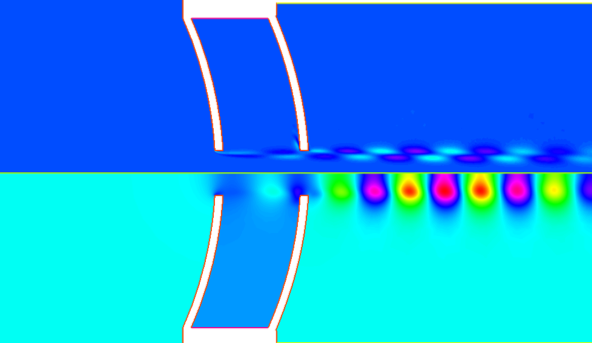
\includegraphics[width=.9\linewidth]{FIGURES/WhistlinJetMode.png}
\end{frame}



\begin{frame}{2D around a spring-mounted cylinder...}
(with Diogo Ferreira Sabino \& Olivier Marquet)
\end{frame}



\begin{frame}{2D flow around a compressible cylinder...}
(in fast progress with Javier Sierra...)
\end{frame}

\begin{frame}{Flow around (and through) a porous (\& rotating) disk...}
(with Adrien Rouvière \& D. Lo Jacono)


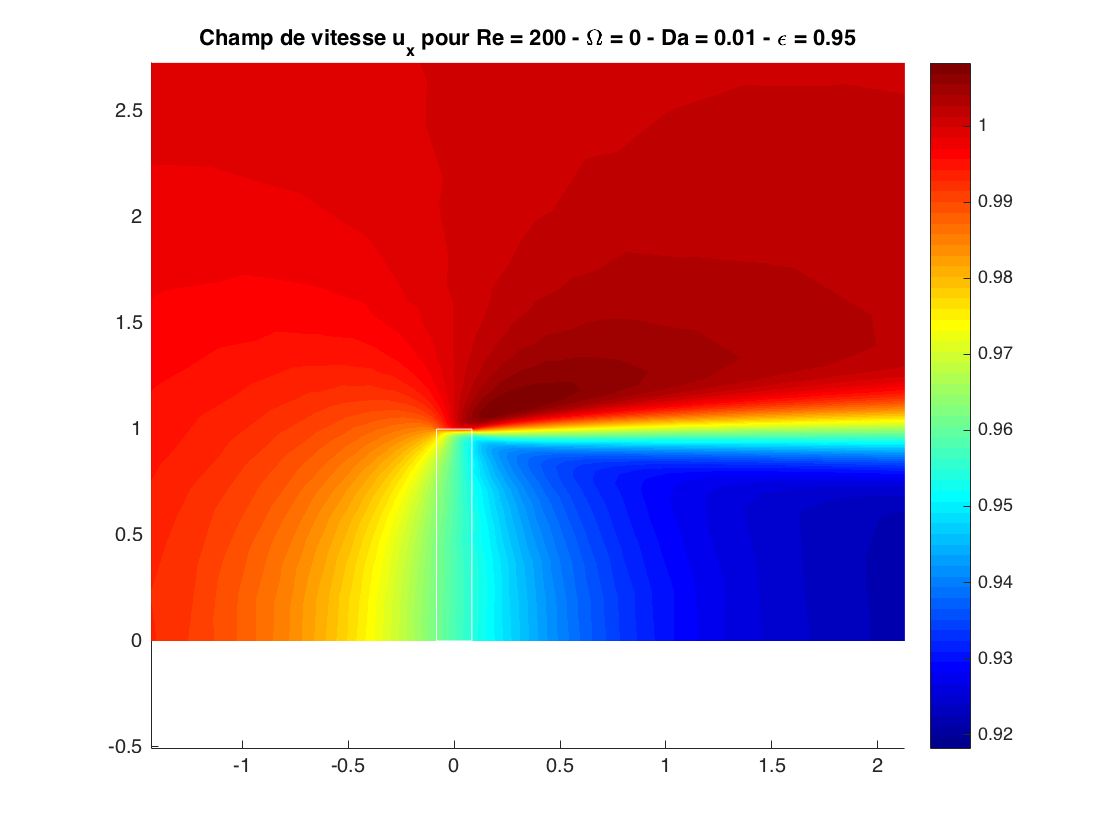
\includegraphics[width=.6\linewidth]{FIGURES/Ux_Re200_Da1e-2.png}

\end{frame}

%%%%%%%%%%%%%%%%%%%%%%%%%%%%%%%%%%%%%%%%%%%%%%%%%%%%%%

\begin{frame}{Liquid bridges...}

\begin{description}
%\item{Directory in the StabFem project :}  \texttt{LiquidBridges}
%\item{Main contributors :} D. Fabre.
\item{Reference :} Chireux et al., Phys. Fluids, 2015.
\end{description}


\begin{figure}
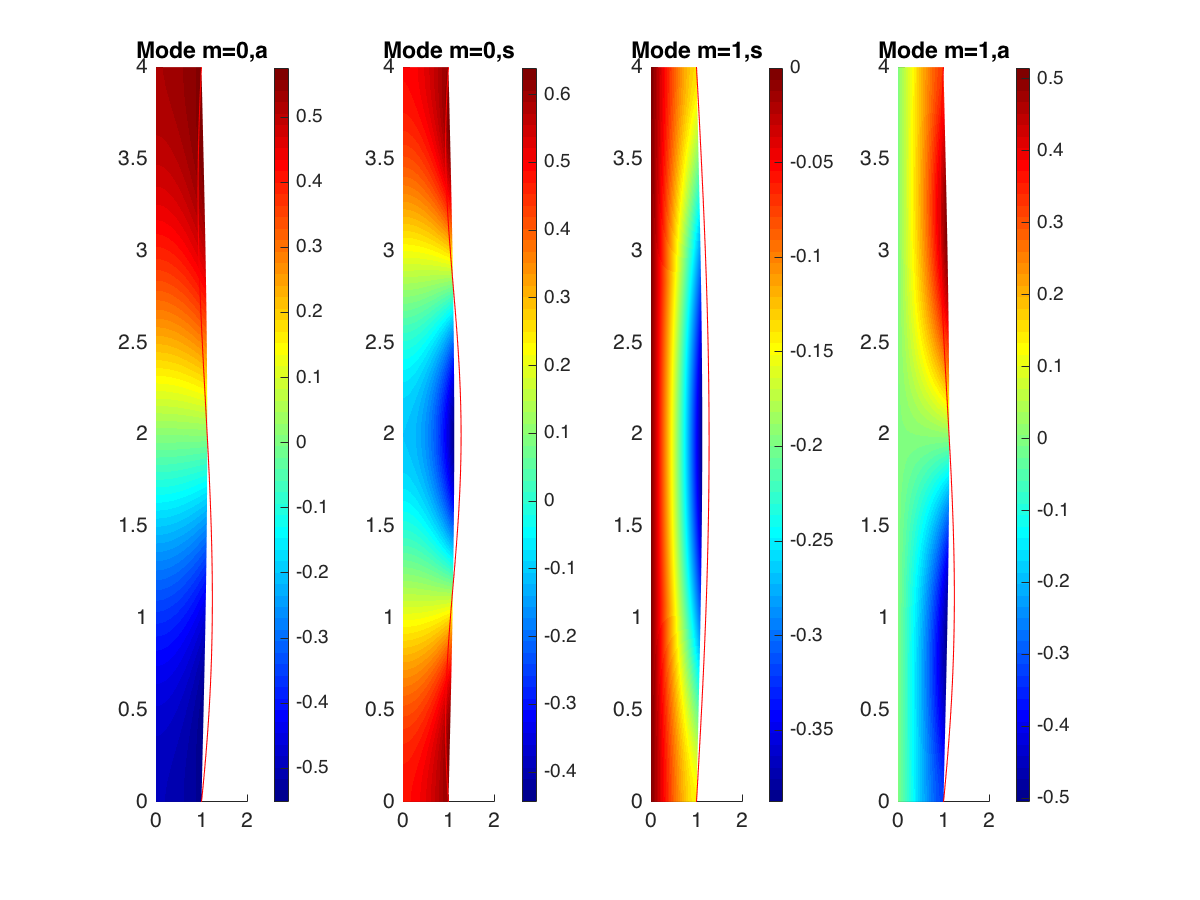
\includegraphics[width=.5\linewidth]{../LiquidBridges/FIGURES/Bridges_NV_Eigenmodes_phi_cyl_L3_5.png}
\caption{Oscillation modes of a liquid bridge of aspect ratio $L/R=4$ and reduced volume $V^ =$...}
\label{Bridges_NV_Eigenmodes_phi_cyl_L3_5}
\end{figure}

\begin{figure}
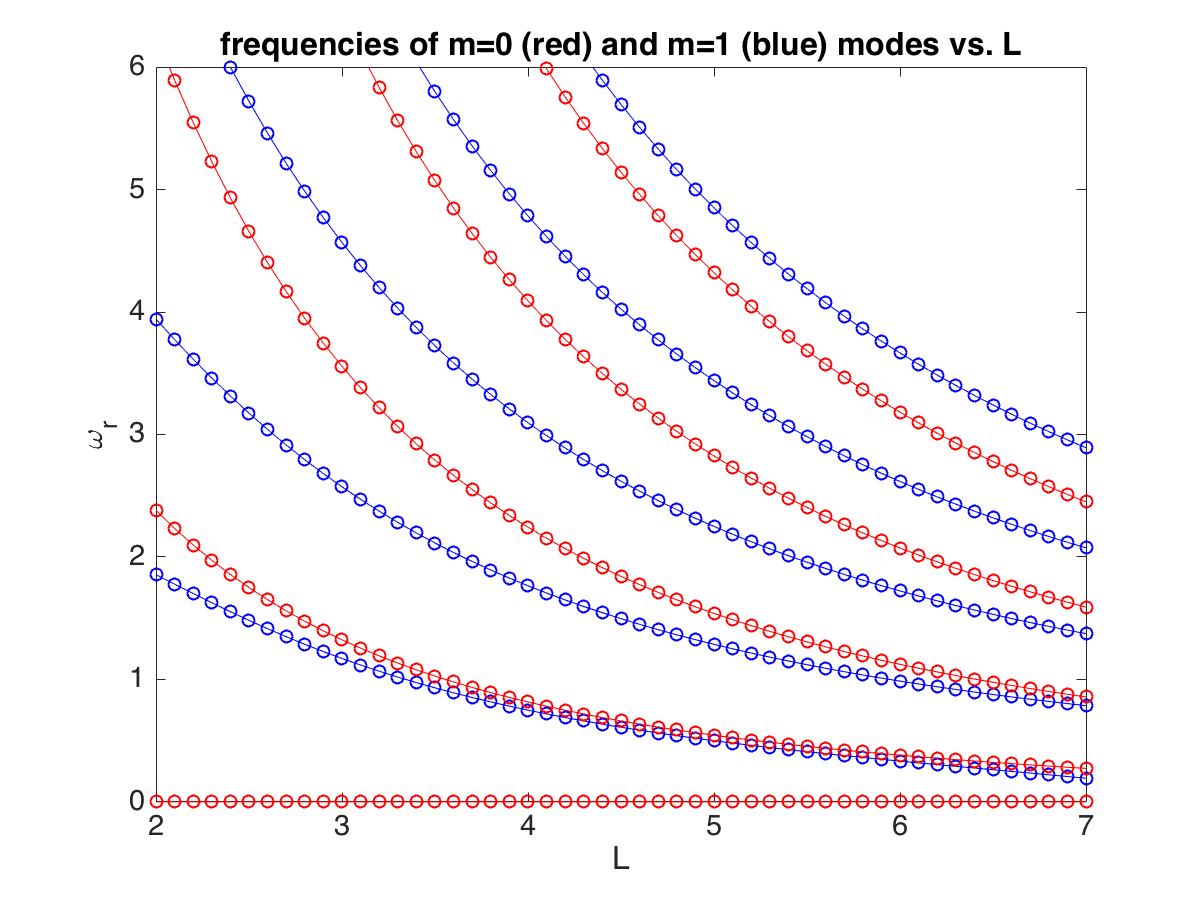
\includegraphics[width=.45\linewidth]{../LiquidBridges/FIGURES/Bridges_NV_coal_omega.png}
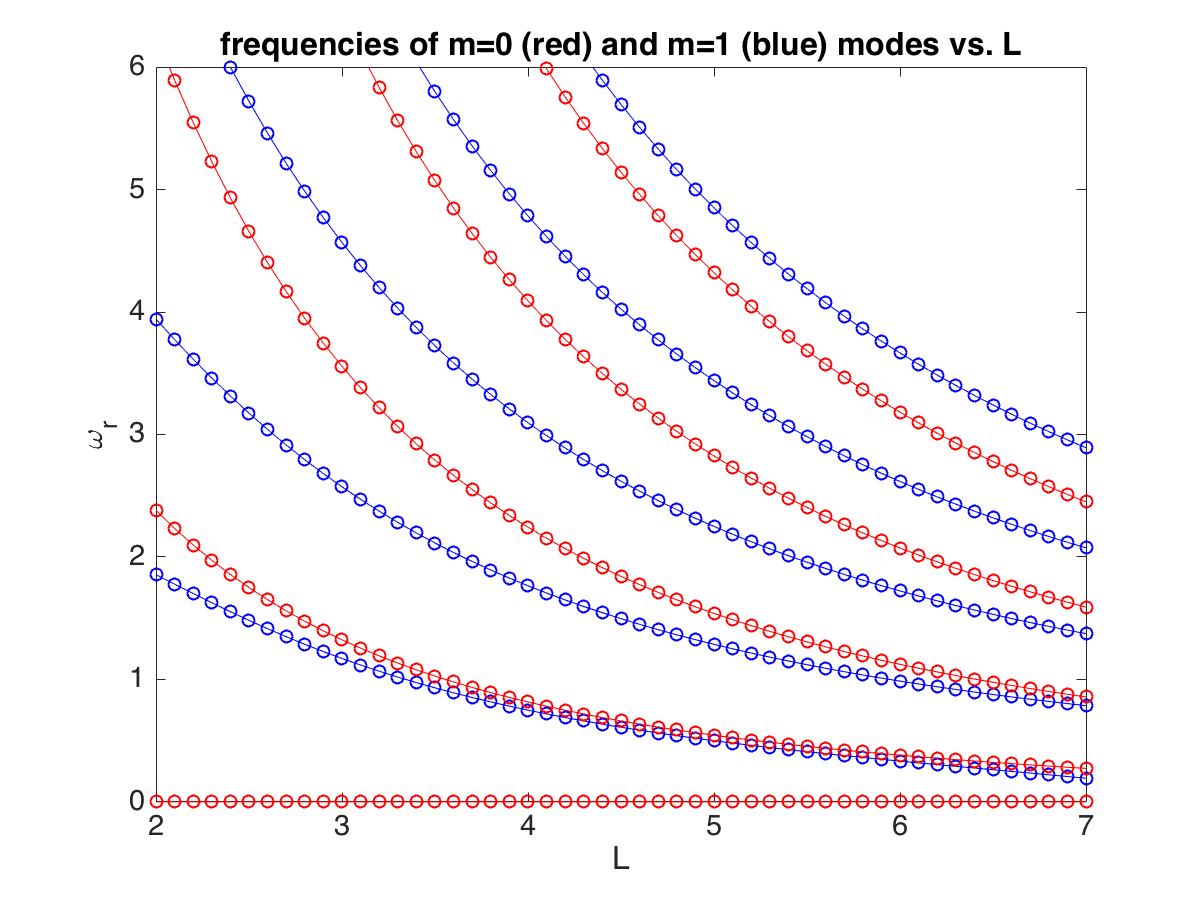
\includegraphics[width=.45\linewidth]{../LiquidBridges/FIGURES/Bridges_NV_coal_omega.png}
\caption{Oscillation frequencies of a liquid bridge resulting from the coalescence of two spherical droplets
as function of $L^* =L/R$
(figures 11,12 of Chireux et al.)
}
\label{Bridges_NV_Eigenmodes_phi_cyl_L3_5}
\end{figure}


\end{frame}


\begin{frame}{rotating polygons...}

\begin{description}
%\item{Directory in the StabFem project :}  \texttt{ROTATINGPOLYGONS}
%\item{Main contributors :} J. Mougel, D. Fabre
\item{Reference :} Mougel et al., JFM 2018 
\end{description}

\begin{figure}
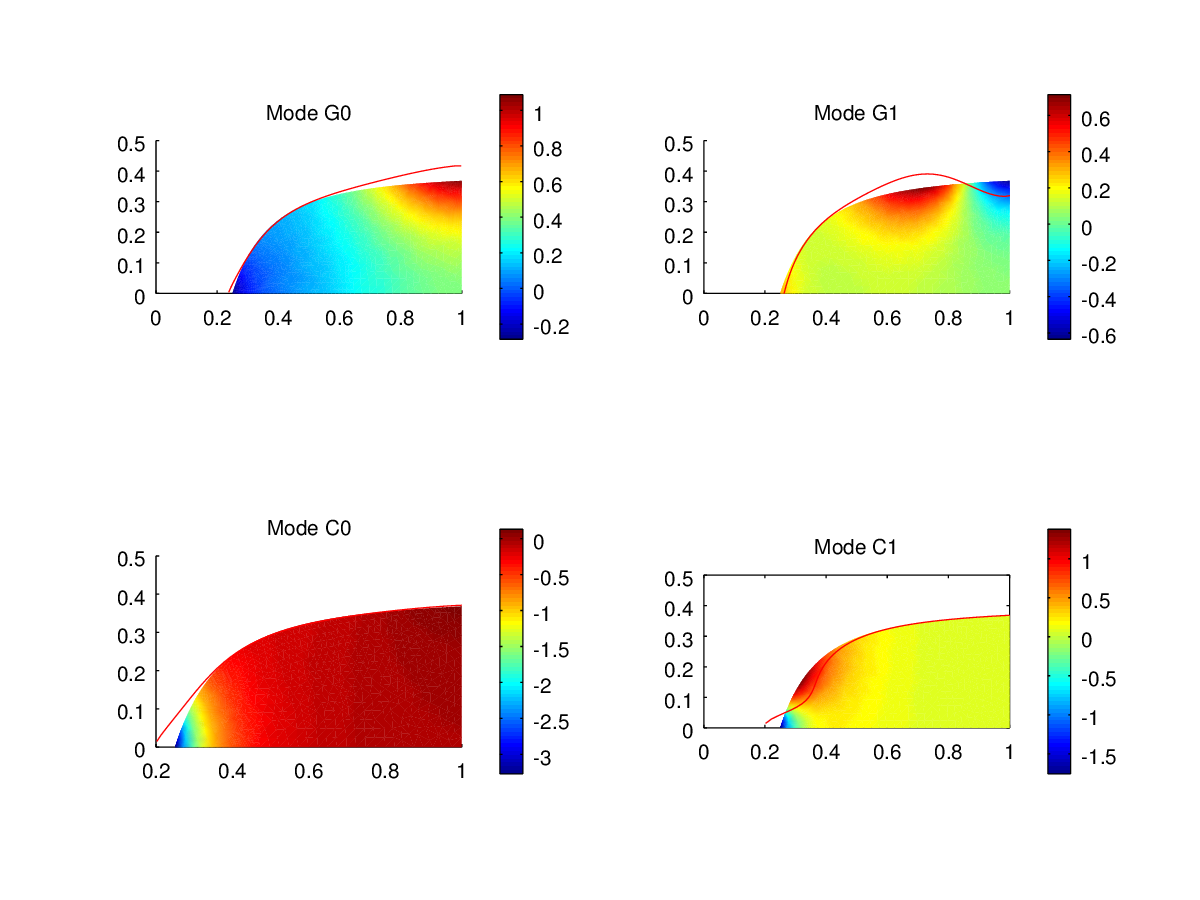
\includegraphics[width=.8\linewidth]{../ROTATING_POLYGONS/FIGURES/POLYGONS_modes.png}
\caption{Oscillation modes of a potential vortex for  $a=H/R=0.3$ and $m=3$ (figure 5, 6 of Mougel et al.).}
\label{Bridges_NV_Eigenmodes_phi_cyl_L3_5}
\end{figure}

\begin{figure}
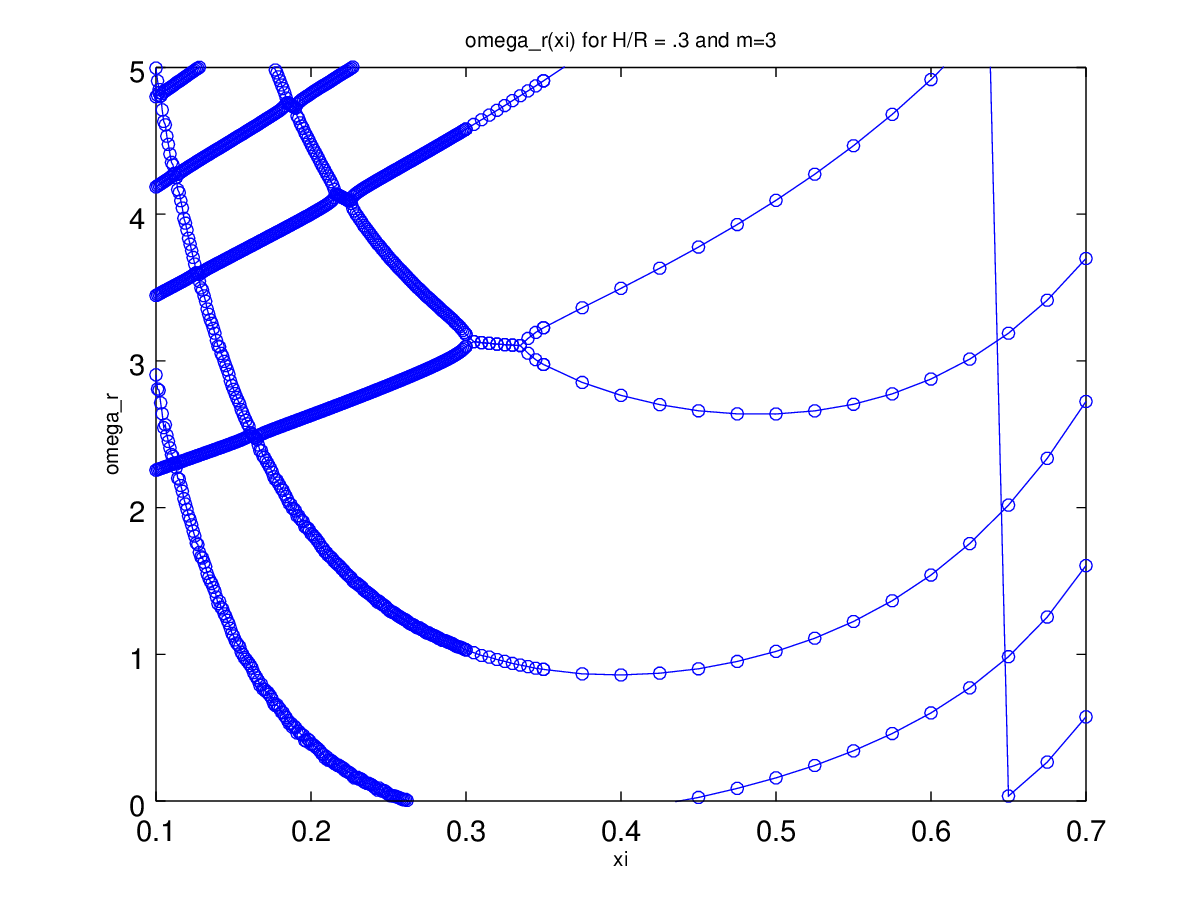
\includegraphics[width=.45\linewidth]{../ROTATING_POLYGONS/FIGURES/POLYGONS_omega.png}
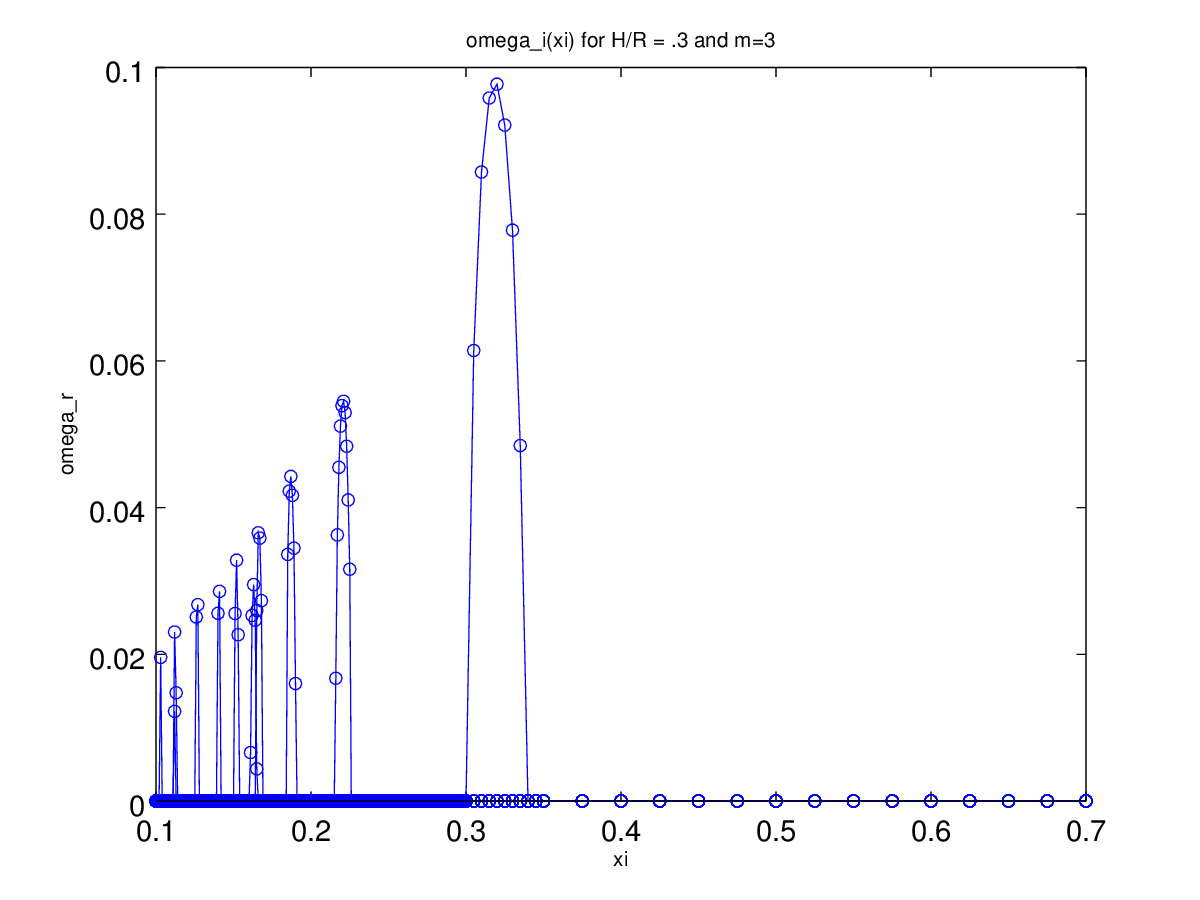
\includegraphics[width=.45\linewidth]{../ROTATING_POLYGONS/FIGURES/POLYGONS_sigma.png}
\caption{Oscillation frequencies and amplification rates for f a potential vortex for $m=3$ (figure 4 of Mougel et al.).}
\label{Bridges_NV_Eigenmodes_phi_cyl_L3_5}
\end{figure}
 
\end{frame}

\begin{frame}{Sessile drops...}

With Nabil Achour  ( \& Paul Bonnefis)

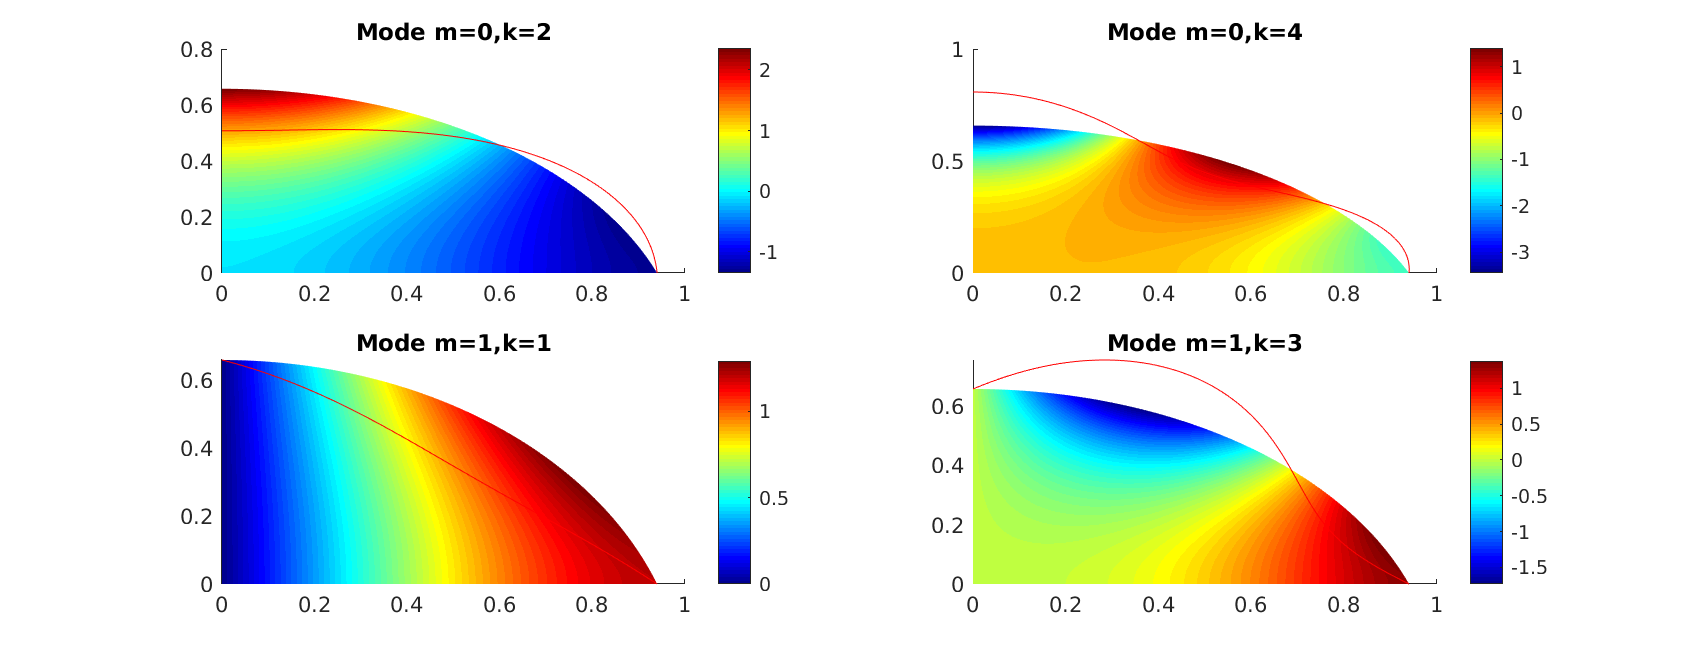
\includegraphics[width=.9\linewidth]{FIGURES/SessileDrops_Eigenmodes.png}     % SessileDrops__Eigenmodes_eta.png

- Linear oscillations modes ("pined" or "fixed angle" conditions)

Next steps : investigate contact-line dynamics with WNL methods (cf. Viola, Brun \& Gallaire, 2018)

\end{frame}



%%%%%%%%%%%%%%% PART 3 : NONLINEAR APPROACHES %%%%%%%%%%%%%%%%%%%

\section{Nonlinear global stability approaches : status and future}


%\section{Nonlinear global approaches to hydrodynamic instabilities}

\begin{frame}{Nonlinear global stability approaches : review}
\small

The linear stability approach approach is the right tool to predict instability threshold ($Re_c$) and the shedding frequency at threshold ($St_c = \omega_c/2\pi$).

\ssp
 But for $Re>Re_c$ it badly predicts the frequency of the limit cycle. 
 
$$
\includegraphics[width=8cm]{Barkley_figure.png}
$$

 
 
 \ssp It has been remarked that stability analysis of the {\em mean flow} obtained by time-averaging the limit cycle gives better predictions (Barkley, Leontini,...).
  
  
\ssp 

  
  => Objective of nonlinear stability approaches : provide rational approach to describe the nonlinear oscillation cycle,
  and provide amplitude equations to describe the transients.
  
  %Give a rigorous ground to study the stability of {\em mean flow}.
  
  

\end{frame}
\subsection{Weakly nonlinear approach}


\begin{frame}{Weakly nonlinear approach {\small (Sipp \& Lebedev, 2007)}}

\footnotesize

Starting point : weakly non-linear expansion, with multiple scale method.

$$
\epsilon = \frac{1}{Re_c} - \frac{1}{Re} ; \quad \tau = \epsilon^2 t
$$

\begin{eqnarray}
{\bf u} &=& {\bf u}_{bc} + \epsilon \left[ A_{wnl} (\tau) \hat{\bf u} e^{i \omega_c t} + c.c. \right] \label{WNL1}\\
&+& \epsilon^2 \left[ {\bf u}_\epsilon + |A_{wnl}|^2  {\bf u}_{2,0} + \left(  A_{wnl}^2 {\bf u}_{2,2} e^{2 i \omega_c t} + c.c. \right) \right] + {\cal O}( \epsilon ^3)
\nonumber
\end{eqnarray}

Resolution at order 2 :
%Substituting the expansion \ref{WNL2} into the Navier-Stokes equations \ref{NSprimitive} and grouping terms multiplied by the same power of $\epsilon$, a hierarchy of equations is obtained. The order $\epsilon^0$ gives directly the base flow at $Re_c$. The order $\epsilon^1$
%corresponds to the linear neutral eigenmode as computed in the first part of this article.
%The order $\epsilon^2$ contains three terms respectively computed as the solutions of the following linear problems:
\begin{eqnarray}
 {\cal LNS}_{{\bf u}_{bc}} ({\bf u}_\epsilon) - 2 \nabla \cdot {\mathsf D}({\bf u}_{bc}) &=&0,
\label{eq:LL1} \\
{\cal LNS}_{{\bf u}_{bc}} ({\bf u}_{2,0}) &=& {\cal C}(\hat{\bf u},\overline{\hat{\bf u}}), \label{eq:LL2} \\
{\cal LNS}_{{\bf u}_{bc}} ({\bf u}_{2,2}) - 2 i \omega_c {\bf u}_{2,2}  &=& \frac{1}{2} {\cal C}(\hat{\bf u},\hat{\bf u}). \label{eq:LL3}
 \end{eqnarray}

Compatibility conditions at order 3 :
\be{WNL3_2}
\frac{\partial A_{wnl}}{\partial \tau} = \Lambda A_{wnl} - (\nu_0+\nu_2)  |A_{wnl}|^2 A_{wnl},
\ee
%where coefficients $\Lambda$, $\nu_0$ and $\nu_2$ are given by
\begin{eqnarray}
\Lambda &=& -\frac{ \left< {\hat{\bf u}}^\dag, 
\left( {\cal C}({\bf u}_\epsilon, \hat{\bf u}) + 2 \nabla \cdot  {\mathsf D}( \hat{\bf u}) \right) \right>}
{  \left<  \hat{\bf u}^\dag,\hat{\bf u} \right> },\label{LAMBDA}\\
\nu_0 &=& \frac{ \left< {\hat{\bf u}}^\dag,  {\cal C}({\bf u}_{20}, \hat{\bf u} ) \right>}
{  \left<  \hat{\bf u}^\dag,\hat{\bf u} \right> },\label{NU0}\quad
\nu_2 = \frac{ \left< {\hat{\bf u}}^\dag,  {\cal C}({\bf u}_{22}, \overline{\hat{\bf u}})  \right>}
{  \left<  \hat{\bf u}^\dag,\hat{\bf u} \right> }.,\label{NU2}
 \end{eqnarray}




%Method : weakly nonlinear expansion

%Order 0 : base-flow

%Order 1 : eigenmode at marginal conditions 

%Order 2 : nonresonant linear problems -> direct resolution

%Order 3 : resonant problems : compatibility conditions (Fredholm alternative)

%Resolution thanks to adjoint methods 

%=> Amplitude equation


\end{frame}

\subsection{Self-consistent approach}


\begin{frame}{Self-Consistent approach {\small (Mantic-Lugo, Arratia \& Gallaire, 2014)}}

\small
Starting point : Pseudo-eigenmode decomposition

\be{SC}
{\bf u } = {\bf u }_m + A_{sc} \left[ \tilde{{\bf u }}_1 e^{\sigma_{sc} t + i \omega_{sc} t} +   \overline{\tilde{\bf u }_1} e^{\sigma_{sc} t  -i \omega_{sc} t} \right],
\quad
\left( |\tilde{{\bf u }}_1|| = 1/\sqrt{2}\right)
\ee  

%where ${\bf u }_m$ is the {\em mean flow} as previously defined,  $\tilde{{\bf u }}_1$ is a pseudo-eigenvector which is normalized by the condition  $||\tilde{{\bf u }}_1|| = 1/\sqrt{2}$, $\overline{\tilde{{\bf u }}_1}$ is its complex conjugate,
where $A_{sc}$ is an amplitude parameter, %directly related to the energy of the oscillating flow, 
and $\lambda_{sc} = \sigma_{sc} + i \omega_{sc}$ is a pseudo-eigenvalue which depends upon the parameter $A_{sc}$. 

\pause
=> SC-model equations

\begin{subequations}\label{sc12}
\begin{eqnarray}
{\cal NS}(  {\bf u }_m ) - A_{sc}^2 {\cal C}( \tilde{{\bf u }}_1, \overline{\tilde{\bf u }_1}) = 0, 
\label{sis1}
\\
(\sigma_{sc} + i \omega_{sc}) \tilde{{\bf u }}_1 =  {\cal LNS}_{{\bf u }_m}(\tilde{{\bf u }}_1 ).
\label{sis2}
\end{eqnarray}
\end{subequations}

\pause

=> Amplitude equation :
$$
\frac{\partial A_{sc}}{\partial t} = \sigma_{sc} (A_{sc}) A_{sc}
$$

\pause

%$\sigma(A_E

Resolution method of {\small (Mantic-Lugo 2014)}: double iterative loop

- Inner loop : 

$\quad$ Fix $A_{sc}$, iteratively solve (eigenvalue problem + calculation of mean flow) up to convergence for $(\sigma_{sc} + i \omega_{sc})$ as function of $A_{sc}$.

- Outer loop : 

$\quad$ iterate over $A_{sc}$ to reach  $\sigma_{sc} = 0$





\end{frame}



\begin{frame}{Self-Consistent approach : a direct resolution method}

\small

Let's forget about transients, and look directly for a description of the saturated cycle:
%We thus start with a truncated Fourier decomposition of the limit cycle under the form:

\be{HB}
{\bf u } = {\bf u }_m + {\bf u }_{1,c} \cos( \omega t ) +   {\bf u }_{1,s} \sin( \omega t ),
\ee
where ${\bf u }_{1,c}$ and ${\bf u }_{1,s}$ are two {\em real} fields %describing the nonlinear perturbation at two instants separated by a quarter-period of oscillation, 

and $\omega$ is the (real) oscillation frequency of the limit cycle.
%The connection with the definition of Manti\v{c}-Lugo is as follows :
%\be{HBtoSC}
%\left( {\bf u }_{1,c} - i {\bf u }_{1,s} \right) = 2 A_{sc} \tilde{{\bf u }}_1.
%\ee 

\ssp
 
=> Equations :
%Injecting this ansartz into the Navier-Stokes equations and taking the mean value and the first Fourier component leads to the following coupled equations:
\begin{subequations}\label{eq_principal}
\begin{eqnarray}
{\cal NS}(  {\bf u }_m ) = \frac{{\cal C}( {\bf u }_{1,c}, {\bf u }_{1,c}) +{\cal C}( {\bf u }_{1,s}, {\bf u }_{1,s})}{4}, 
\label{HBEq0}
\\
 \omega {\bf u }_{1,s} =  {\cal LNS}_{{\bf u }_m}(  {\bf u }_{1,c} ),
\label{HBEq1}
\\
 -\omega {\bf u }_{1,c} =  {\cal LNS}_{{\bf u }_m}(  {\bf u }_{1,s} ).
\label{HBEq1b}
\end{eqnarray}
\end{subequations}

We need an extra scalar equation to fix the phase of the cycle, e.g:

\begin{equation}
\Im \{F_y({\bf u}_1) \} =0.
\label{HBphase}
\end{equation}

=> Direct resolution with Newton method !
\ssp


Remarks :

- We need a good guess : use the WNL to produce it !

- Computation can be optimized using preconditioning (Ask Olivier...)

\end{frame}


\subsection{Harmonic-balance approach}


\begin{frame}{Harmonic-Balance}

\small

%The Navier-stokes equations can be posed as

%\begin{eqnarray}
%\partial_t {\bf u} = {\cal NS} ({\bf u},p)
%\equiv - {\bf u} \cdot \nabla {\bf u} - \nabla p + \frac{2}{Re}  \nabla \cdot {\mathsf{D}}({\bf u}), \label{NSprimitive}  \\
%\nabla \cdot {\bf u} = 0. \label{eq:DIV}
%\end{eqnarray}


We start with the following expansion:
\begin{equation}
{\bf u } = {\bf u }_m + {\bf u }_{1,c} \cos( \omega t ) +   {\bf u }_{1,s} \sin( \omega t ) +{\bf u }_{2,c} \cos(2 \omega t ) +   {\bf u }_{2,s} \sin(2 \omega t ),
\end{equation}

arriving to a system of equations:
\begin{subequations}\label{eq_principal}
\begin{eqnarray}
{\cal NS}(  {\bf u }_m) = \frac{{\cal C}( {\bf u }_{1,c}, {\bf u }_{1,c}) +{\cal C}( {\bf u }_{1,s}, {\bf u }_{1,s})+{\cal C}( {\bf u }_{2,c}, {\bf u }_{2,c})+{\cal C}( {\bf u }_{2,s}, {\bf u }_{2,s})}{4}, 
\label{HBEq0}
\\
 \omega {\bf u }_{1,s} =  {\cal L}_{{\bf u }_m}(  {\bf u }_{1,c} )-\frac{1}{2}\Big(
 {\cal C}( {\bf u }_{1,c}, {\bf u }_{2,c})+{\cal C}( {\bf u }_{1,s}, {\bf u }_{2,s})
 \Big),
\label{HBEq1}
\\
 -\omega {\bf u }_{1,c} =  {\cal L}_{{\bf u }_m}(  {\bf u }_{1,s} )-\frac{1}{2}\Big(
 {\cal C}( {\bf u }_{1,c}, {\bf u }_{2,s})-{\cal C}( {\bf u }_{1,s}, {\bf u }_{2,c})
 \Big),
\label{HBEq1b}
\\
 2 \omega {\bf u }_{2,s} =  {\cal L}_{{\bf u }_m}(  {\bf u }_{2,c} )-\frac{1}{4}\Big(
 {\cal C}( {\bf u }_{1,c}, {\bf u }_{1,c})-{\cal C}( {\bf u }_{1,s}, {\bf u }_{1,s})
 \Big),
\label{HBEq2}
\\
 -2\omega {\bf u }_{2,s} =  {\cal L}_{{\bf u }_m}(  {\bf u }_{2,s} )-\frac{1}{2}
 {\cal C}( {\bf u }_{1,s}, {\bf u }_{1,c}),
\label{HBEq2b}
\end{eqnarray}
\end{subequations}
%where ${\cal C}( {\bf U} , {\bf u}) = \left( {\bf U} \cdot \nabla \right) {\bf u} + \left( {\bf u} \cdot \nabla \right)  {\bf U}$. 

%To allow resolution we thus need an extra equation to fix this phase, e.g:
\begin{equation}
\Im \{F_y({\bf u}_1) \} =0.
\label{HBphase}
\end{equation}

=> Direct Newton resolution again
\end{frame}


\begin{frame}{Harmonic-Balance : results for the cylinder ! }

%\begin{figure}
\begin{center}
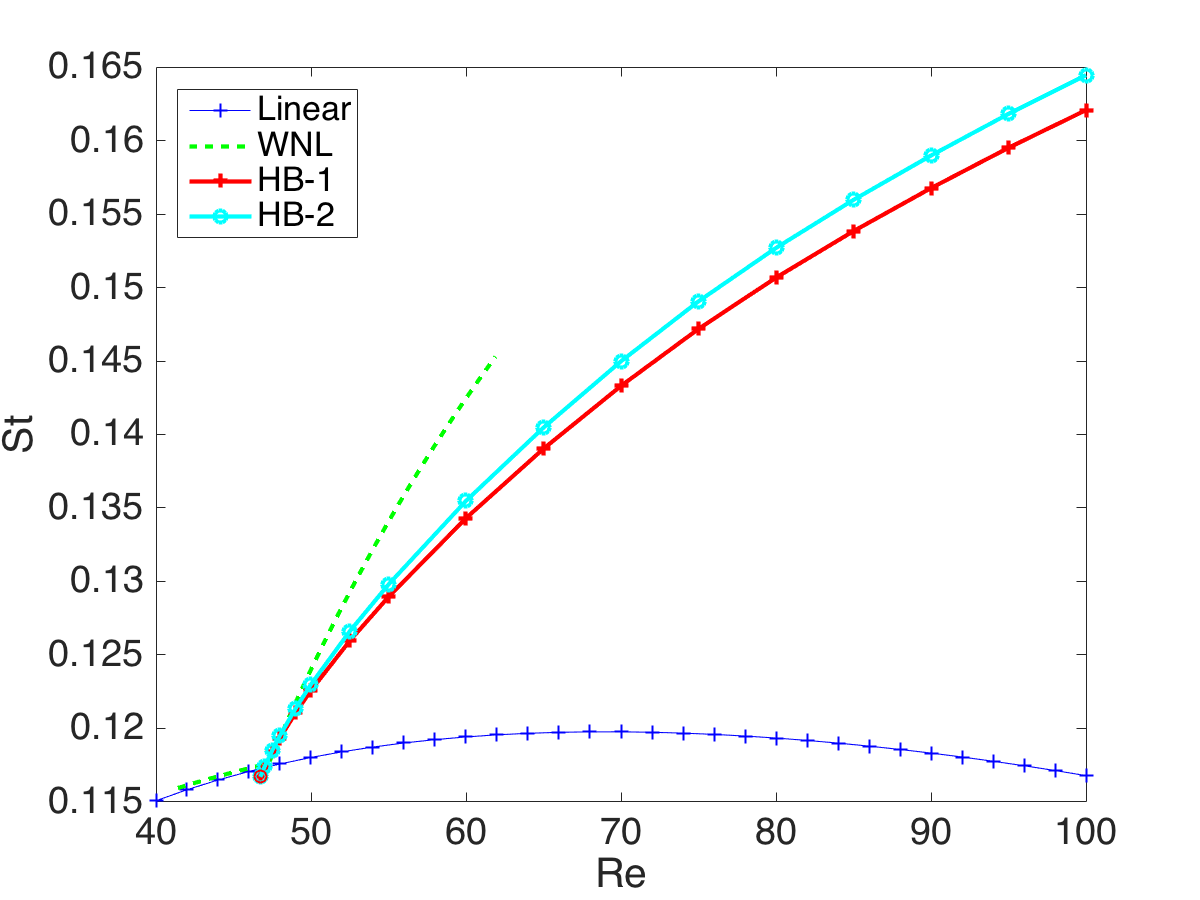
\includegraphics[width=.32 \linewidth]{../CYLINDER/FIGURES/Cylinder_Strouhal_Re_HB2.png}
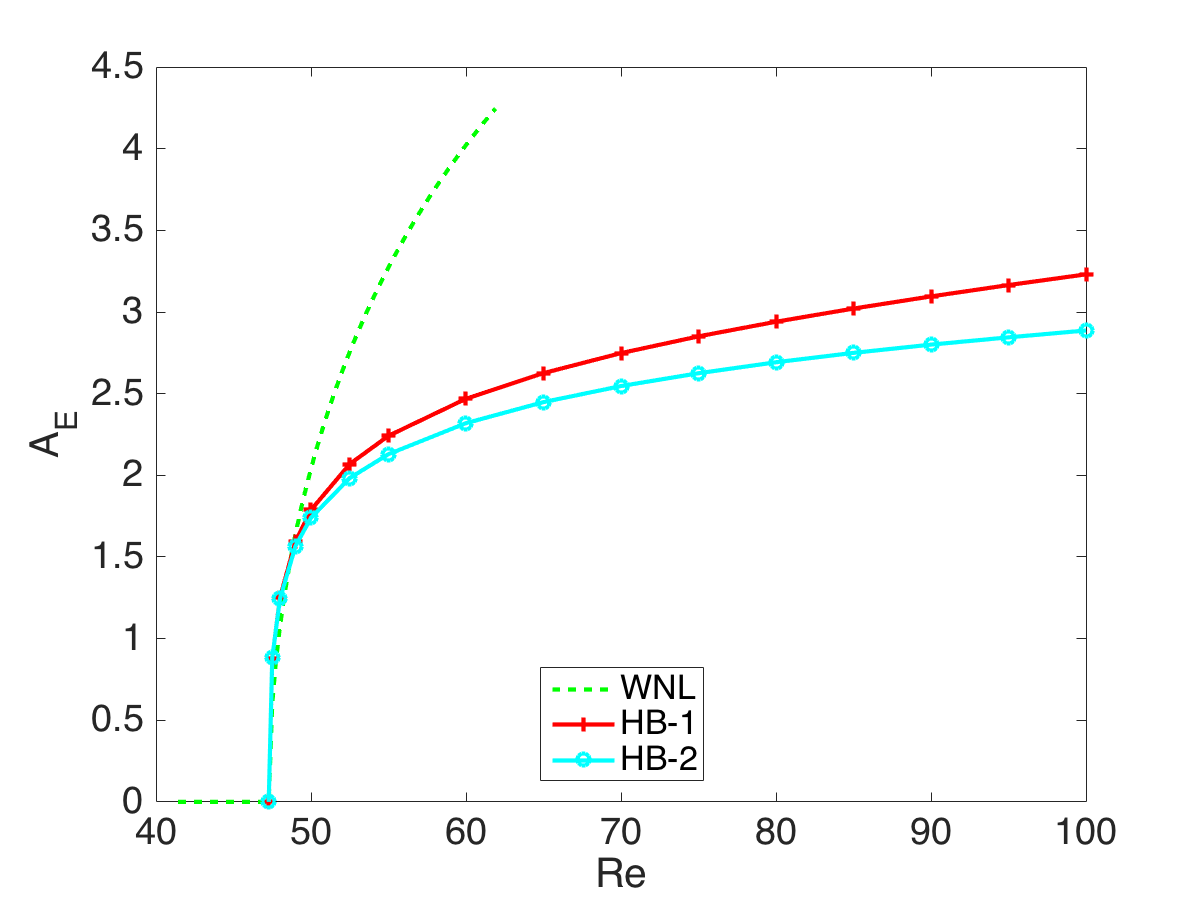
\includegraphics[width=.32 \linewidth]{../CYLINDER/FIGURES/Cylinder_Energy_Re_HB2.png}
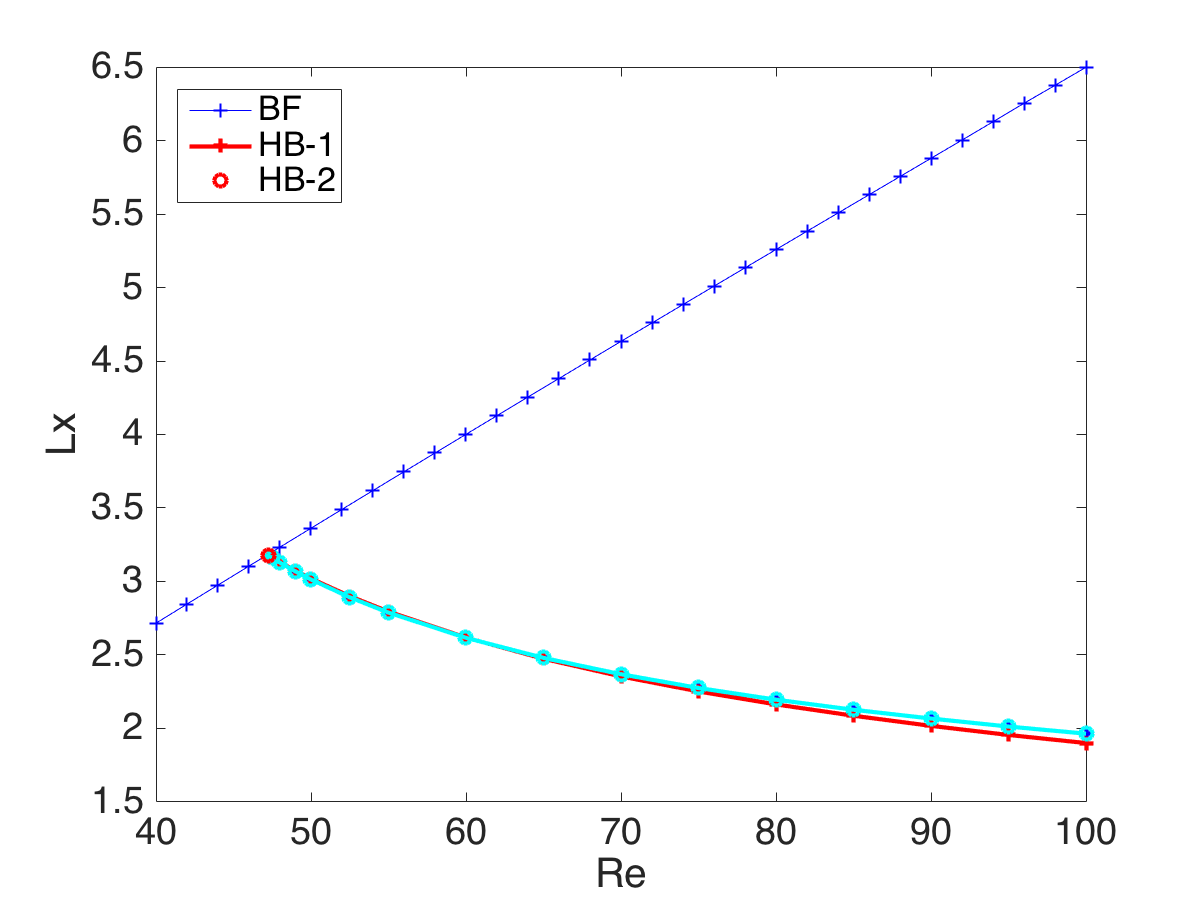
\includegraphics[width=.32 \linewidth]{../CYLINDER/FIGURES/Cylinder_Lx_Re_HB2.png}
\end{center}
\begin{center}
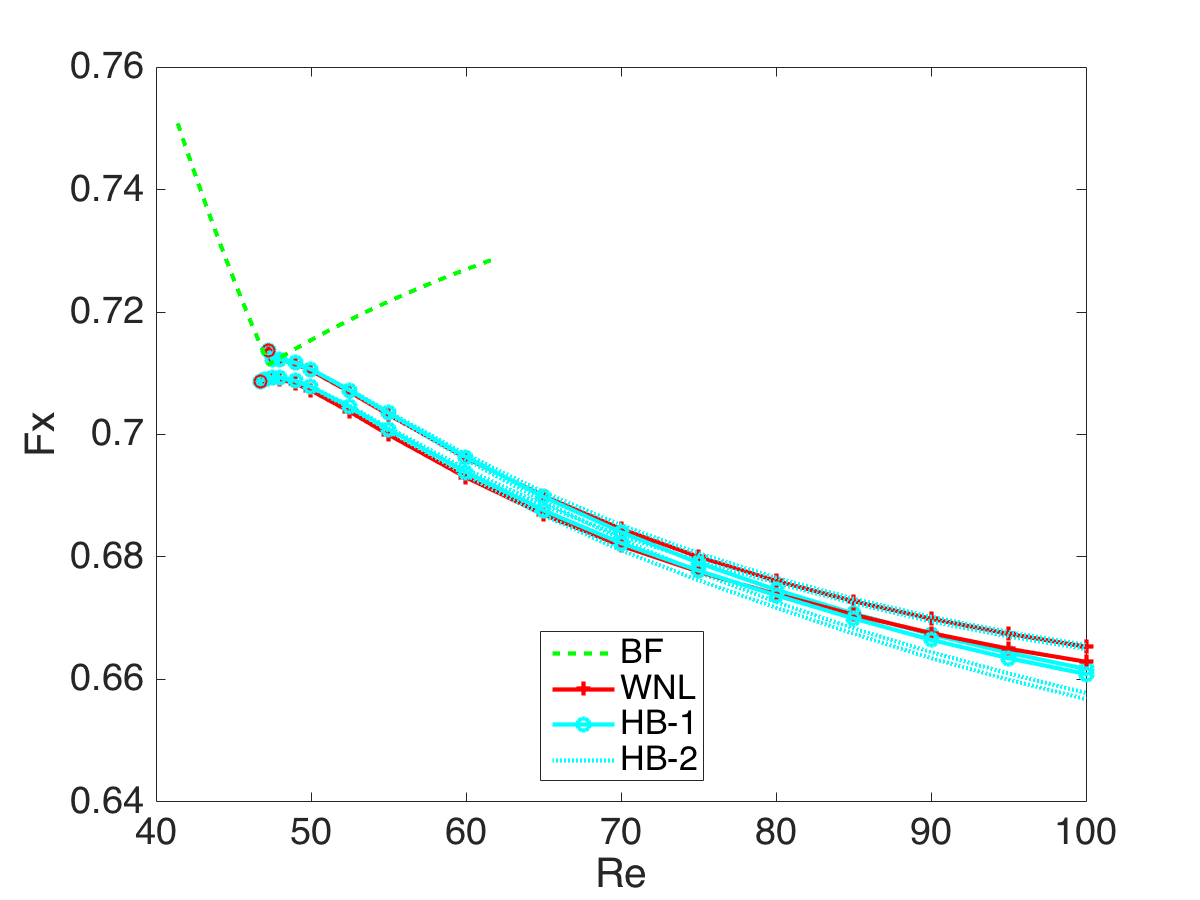
\includegraphics[width=.32\linewidth]{../CYLINDER/FIGURES/Cylinder_Fx_Re_HB2.png}
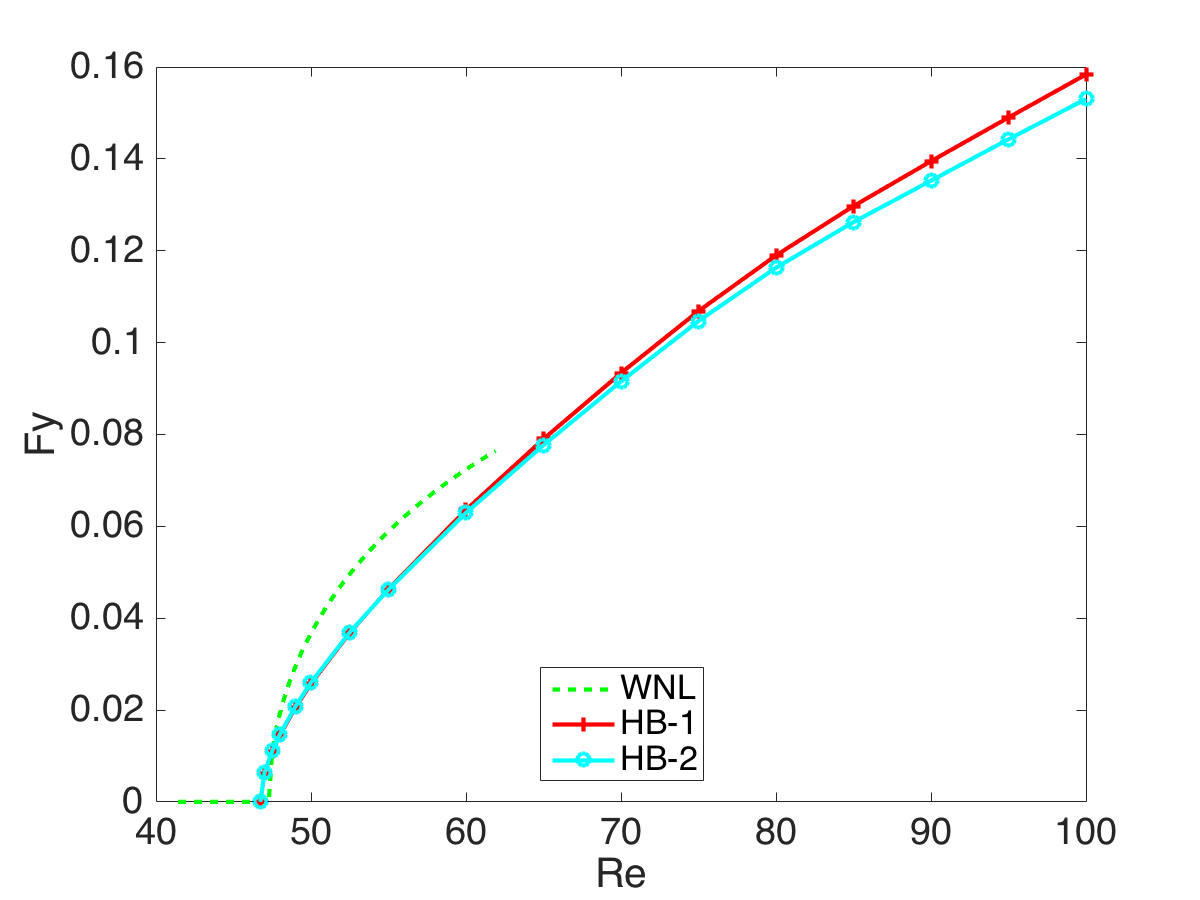
\includegraphics[width=.32 \linewidth]{../CYLINDER/FIGURES/Cylinder_Fy_Re_HB2.png}
\end{center}
%\caption{Comparison between the weakly nonlinear results (WNL) the harmonic balance data (HB), and baseflow/linear results : Strouhal number $(a)$, Mean drag $(b)$, amplitude of oscillating lift $(c)$, Energy-amplitude of the nonlinear perturbation $(d)$ and recirculation lenght of mean/base flows ($e)$. 
%c_x should be consistent with the drag definition given at beginning
%}
%\label{fig:HB_SC_DATA_COMP}
%\end{figure}

\end{frame}

%
%\subsection{Adjoint problem} 
%
%\begin{frame}{Adjoint problem}
%
%\small
%
%Define a scalar product :
%$$
%\left< \phi_1, \phi_2 \right> = \int_\Omega \overline{\phi_1} \cdot \phi_2   \mbox{ d} \Omega
%$$
%
%
%We can first define the {\em adjoint linearised Navier-Stokes operator} $NSL^\dag$ defined by the property:
%\bes{NSLAdj}
%\forall ( {\bf u}, p ; {\bf v}, q), & \left< NSL^\dag_{\bf U}( {\bf v},q) ,{\bf u}\right> + \left< \nabla \cdot {\bf v},p\right>  \\
%=& \left< {\bf v}, NSL_{\bf U} ({\bf u},p)\right> + \left< q, \nabla \cdot {\bf u}\right>.
%\ees
%We can then define the adjoint eigenmodes as the solutions to the eigenvalue problem 
%\be{EigenAdj} 
%\forall ( {\bf u}, p), \quad  \lambda^\dag \left< \hat{\bf v}, {\bf u}\right> =
% \left< NSL^\dag_{\bf U}( \hat{\bf v},\hat{q}) ,{\bf u}\right> + \left< \nabla \cdot \hat{\bf v},p\right>  
%\ee
%
%Matricial form :
%
%\be{Eigen_Adj_matricial}
%\overline{\lambda}^\dag B \hat{X}\dag = A^T \hat{X}\dag.
%\ee
%
%
%\end{frame}
%
%\begin{frame}{Adjoint mode and structural sensitivity}
%
%
%Significance of the adjoint mode : 
%
%(optimal perturbation)
%
%
%\end{frame}

%\section{Nonlinear global approaches to hydrodynamic instabilities}
%
%\begin{frame}{Nonlinear global stability approaches : review}
%
%%The linear stability approach approach is the right tool to predict instability threshold ($Re_c$) and the %shedding frequency at threshold ($St_c = \omega_c/2\pi$).
%
%%\ssp
%% But for $Re>Re_c$ it badly predicts the frequency of the limit cycle. 
% 
%%$$
%%\includegraphics[width=8cm]{FIGURES/Barkley_figure.png}
%%$$
%
% 
% 
%% \ssp It has been remarked that stability analysis of the {\em mean flow} obtained by time-averaging the limit cycle gives better predictions (Barkley, Leontini,...).
%  
%  
%%\ssp 
%  
% % => Objective of nonlinear stability approaches : Give a rigourous ground to study the stability of mean flow.
%  
%  
%
%\end{frame}
%
%\begin{frame}{Weakly nonlinear approach {\small (Sipp \& Lebedev, 2007)}}
%
%Starting point : weakly non-linear expansion, with multiple scale method.
%
%$$
%\epsilon : \frac{1}{Re_c} - \frac{1}{Re} ; \quad \tau = \epsilon^2 t
%$$
%
%\begin{eqnarray}
%{\bf u} &=& {\bf u}_{bc} + \epsilon \left[ A_{wnl} (\tau) \hat{\bf u} e^{i \omega_c t} + c.c. \right] \label{WNL1}\\
%&+& \epsilon^2 \left[ {\bf u}_\epsilon + |A_{wnl}|^2  {\bf u}_{2,0} + \left(  A_{wnl}^2 {\bf u}_{2,2} e^{2 i \omega_c t} + c.c. \right) \right] + {\cal O}( \epsilon ^3)
%\nonumber
%\end{eqnarray}
%
%
%\end{frame}
%
%
%
%\begin{frame}{Self-Consistent approach {\small (Mantic-Lugo, Arratia \& Gallaire, 2014)}}
%
%Starting point : Pseudo-eigenmode decomposition
%
%
%
%\end{frame}


\begin{frame}{Conclusions}
\end{frame}



\appendix{The future of StabFem }

\begin{frame}{Recent progress}

\begin{itemize}

\item Multi-platform objective : 
MacOs OK ; Unix OK ; Windows 10 currently 50 \% compatible.

{\small main issues with windows : cp = copy,...}%  \verb|\| instead of \verb|/|,...}

\item Plotting options : recent intergration of "pdeplot2dff" from Markus "chloros" in place of pdeplot/pdetools .

{\small other solutions for plotting : tecplot converter, vtk converter, ...}

\item Compatibility with Octave : currently 50 \% compatible.

{\small Main issues with octave : importdata, plotting (now solved), inputParser (now solved)}.

\item Translation in Python  ??

\end{itemize}

\end{frame}




%%%%%%%%%%%%
\begin{frame}{Besoins}

\begin{itemize}

\item Maintaining a fully opensource  (Matlab-Octave or Python ?) and fully multiplatform version (windows).

\item Managing a list of test cases (non-regression tests, etc...)

\item Help simplifying/rationalizing the programation style.

\item Gestion of errors / debugging / "verbosity" ...

\item Upgrading to 3D / parallel computation ? (currently not priority)

\item Support with github  (/ gitlab ?)

\item Documentation 

Automatic generation from comments in programs ?  Doxygen ??


\end{itemize}


\end{frame}




\end{document}

